

\tikzset{every picture/.style={line width=0.75pt}} %set default line width to 0.75pt        

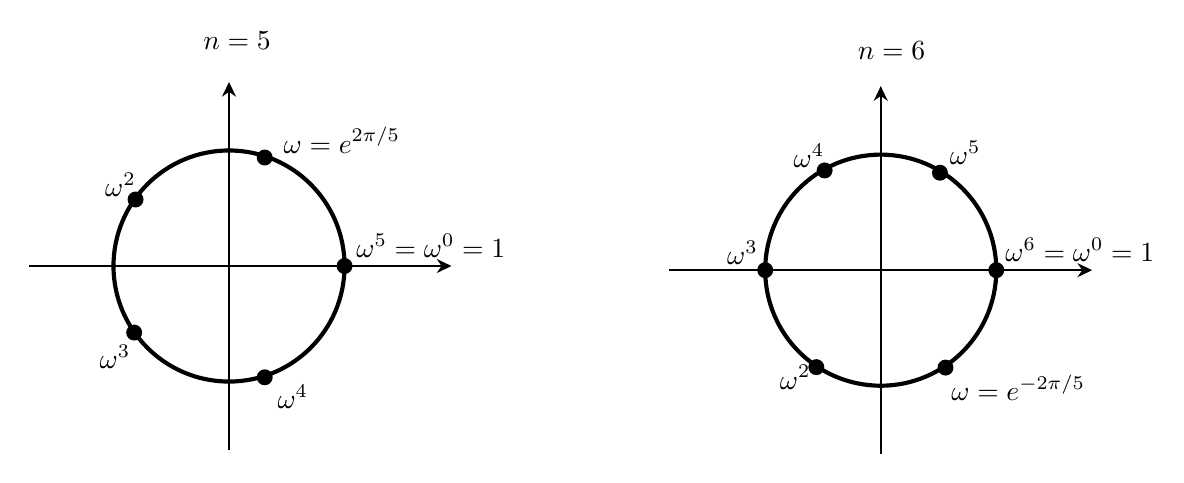
\begin{tikzpicture}[x=0.5pt,y=0.5pt,yscale=-1,xscale=1]
%uncomment if require: \path (0,445); %set diagram left start at 0, and has height of 445

%Straight Lines [id:da8759123208415905] 
\draw [color={rgb, 255:red, 0; green, 0; blue, 0 }  ,draw opacity=1 ][line width=0.75]    (338.52,214.5) -- (36,214.5) ;
\draw [shift={(341.52,214.5)}, rotate = 180] [fill={rgb, 255:red, 0; green, 0; blue, 0 }  ,fill opacity=1 ][line width=0.08]  [draw opacity=0] (10.72,-5.15) -- (0,0) -- (10.72,5.15) -- (7.12,0) -- cycle    ;
%Straight Lines [id:da821272442788836] 
\draw [color={rgb, 255:red, 0; green, 0; blue, 0 }  ,draw opacity=1 ][line width=0.75]    (180.76,84.5) -- (180.76,347.5) ;
\draw [shift={(180.76,81.5)}, rotate = 90] [fill={rgb, 255:red, 0; green, 0; blue, 0 }  ,fill opacity=1 ][line width=0.08]  [draw opacity=0] (10.72,-5.15) -- (0,0) -- (10.72,5.15) -- (7.12,0) -- cycle    ;
%Shape: Circle [id:dp05681939794999513] 
\draw  [line width=1.5]  (97.26,214.5) .. controls (97.26,168.38) and (134.65,131) .. (180.76,131) .. controls (226.88,131) and (264.26,168.38) .. (264.26,214.5) .. controls (264.26,260.62) and (226.88,298) .. (180.76,298) .. controls (134.65,298) and (97.26,260.62) .. (97.26,214.5) -- cycle ;
%Shape: Circle [id:dp3013076520100272] 
\draw  [fill={rgb, 255:red, 0; green, 0; blue, 0 }  ,fill opacity=1 ] (259.26,214.5) .. controls (259.26,211.74) and (261.5,209.5) .. (264.26,209.5) .. controls (267.02,209.5) and (269.26,211.74) .. (269.26,214.5) .. controls (269.26,217.26) and (267.02,219.5) .. (264.26,219.5) .. controls (261.5,219.5) and (259.26,217.26) .. (259.26,214.5) -- cycle ;
%Shape: Circle [id:dp42532911487328906] 
\draw  [fill={rgb, 255:red, 0; green, 0; blue, 0 }  ,fill opacity=1 ] (201.56,136.09) .. controls (201.56,133.33) and (203.8,131.09) .. (206.56,131.09) .. controls (209.33,131.09) and (211.56,133.33) .. (211.56,136.09) .. controls (211.56,138.85) and (209.33,141.09) .. (206.56,141.09) .. controls (203.8,141.09) and (201.56,138.85) .. (201.56,136.09) -- cycle ;
%Shape: Circle [id:dp661891511194406] 
\draw  [fill={rgb, 255:red, 0; green, 0; blue, 0 }  ,fill opacity=1 ] (108.21,166.42) .. controls (108.21,163.66) and (110.45,161.42) .. (113.21,161.42) .. controls (115.97,161.42) and (118.21,163.66) .. (118.21,166.42) .. controls (118.21,169.18) and (115.97,171.42) .. (113.21,171.42) .. controls (110.45,171.42) and (108.21,169.18) .. (108.21,166.42) -- cycle ;
%Shape: Circle [id:dp1005434022322731] 
\draw  [fill={rgb, 255:red, 0; green, 0; blue, 0 }  ,fill opacity=1 ] (201.56,294.91) .. controls (201.56,292.15) and (203.8,289.91) .. (206.56,289.91) .. controls (209.33,289.91) and (211.56,292.15) .. (211.56,294.91) .. controls (211.56,297.67) and (209.33,299.91) .. (206.56,299.91) .. controls (203.8,299.91) and (201.56,297.67) .. (201.56,294.91) -- cycle ;
%Shape: Circle [id:dp9205997842787009] 
\draw  [fill={rgb, 255:red, 0; green, 0; blue, 0 }  ,fill opacity=1 ] (107.21,262.58) .. controls (107.21,259.82) and (109.45,257.58) .. (112.21,257.58) .. controls (114.97,257.58) and (117.21,259.82) .. (117.21,262.58) .. controls (117.21,265.34) and (114.97,267.58) .. (112.21,267.58) .. controls (109.45,267.58) and (107.21,265.34) .. (107.21,262.58) -- cycle ;
%Straight Lines [id:da5753672664447395] 
\draw [color={rgb, 255:red, 0; green, 0; blue, 0 }  ,draw opacity=1 ][line width=0.75]    (801.52,217.5) -- (499,217.5) ;
\draw [shift={(804.52,217.5)}, rotate = 180] [fill={rgb, 255:red, 0; green, 0; blue, 0 }  ,fill opacity=1 ][line width=0.08]  [draw opacity=0] (10.72,-5.15) -- (0,0) -- (10.72,5.15) -- (7.12,0) -- cycle    ;
%Straight Lines [id:da6881124738646721] 
\draw [color={rgb, 255:red, 0; green, 0; blue, 0 }  ,draw opacity=1 ][line width=0.75]    (651.76,87.5) -- (651.76,350.5) ;
\draw [shift={(651.76,84.5)}, rotate = 90] [fill={rgb, 255:red, 0; green, 0; blue, 0 }  ,fill opacity=1 ][line width=0.08]  [draw opacity=0] (10.72,-5.15) -- (0,0) -- (10.72,5.15) -- (7.12,0) -- cycle    ;
%Shape: Circle [id:dp5675892160974338] 
\draw  [line width=1.5]  (568.26,217.5) .. controls (568.26,171.38) and (605.65,134) .. (651.76,134) .. controls (697.88,134) and (735.26,171.38) .. (735.26,217.5) .. controls (735.26,263.62) and (697.88,301) .. (651.76,301) .. controls (605.65,301) and (568.26,263.62) .. (568.26,217.5) -- cycle ;
%Shape: Circle [id:dp7901124514711858] 
\draw  [fill={rgb, 255:red, 0; green, 0; blue, 0 }  ,fill opacity=1 ] (730.26,217.5) .. controls (730.26,214.74) and (732.5,212.5) .. (735.26,212.5) .. controls (738.02,212.5) and (740.26,214.74) .. (740.26,217.5) .. controls (740.26,220.26) and (738.02,222.5) .. (735.26,222.5) .. controls (732.5,222.5) and (730.26,220.26) .. (730.26,217.5) -- cycle ;
%Shape: Circle [id:dp8992653780362201] 
\draw  [fill={rgb, 255:red, 0; green, 0; blue, 0 }  ,fill opacity=1 ] (689.56,147.09) .. controls (689.56,144.33) and (691.8,142.09) .. (694.56,142.09) .. controls (697.33,142.09) and (699.56,144.33) .. (699.56,147.09) .. controls (699.56,149.85) and (697.33,152.09) .. (694.56,152.09) .. controls (691.8,152.09) and (689.56,149.85) .. (689.56,147.09) -- cycle ;
%Shape: Circle [id:dp7236067841601378] 
\draw  [fill={rgb, 255:red, 0; green, 0; blue, 0 }  ,fill opacity=1 ] (606.21,145.42) .. controls (606.21,142.66) and (608.45,140.42) .. (611.21,140.42) .. controls (613.97,140.42) and (616.21,142.66) .. (616.21,145.42) .. controls (616.21,148.18) and (613.97,150.42) .. (611.21,150.42) .. controls (608.45,150.42) and (606.21,148.18) .. (606.21,145.42) -- cycle ;
%Shape: Circle [id:dp5665363843506173] 
\draw  [fill={rgb, 255:red, 0; green, 0; blue, 0 }  ,fill opacity=1 ] (693.56,287.91) .. controls (693.56,285.15) and (695.8,282.91) .. (698.56,282.91) .. controls (701.33,282.91) and (703.56,285.15) .. (703.56,287.91) .. controls (703.56,290.67) and (701.33,292.91) .. (698.56,292.91) .. controls (695.8,292.91) and (693.56,290.67) .. (693.56,287.91) -- cycle ;
%Shape: Circle [id:dp7356242289210358] 
\draw  [fill={rgb, 255:red, 0; green, 0; blue, 0 }  ,fill opacity=1 ] (600.21,287.58) .. controls (600.21,284.82) and (602.45,282.58) .. (605.21,282.58) .. controls (607.97,282.58) and (610.21,284.82) .. (610.21,287.58) .. controls (610.21,290.34) and (607.97,292.58) .. (605.21,292.58) .. controls (602.45,292.58) and (600.21,290.34) .. (600.21,287.58) -- cycle ;
%Shape: Circle [id:dp22660151420836994] 
\draw  [fill={rgb, 255:red, 0; green, 0; blue, 0 }  ,fill opacity=1 ] (563.26,217.5) .. controls (563.26,214.74) and (565.5,212.5) .. (568.26,212.5) .. controls (571.02,212.5) and (573.26,214.74) .. (573.26,217.5) .. controls (573.26,220.26) and (571.02,222.5) .. (568.26,222.5) .. controls (565.5,222.5) and (563.26,220.26) .. (563.26,217.5) -- cycle ;

% Text Node
\draw (160,43) node [anchor=north west][inner sep=0.75pt]   [align=left] {$\displaystyle n=5$};
% Text Node
\draw (633,50) node [anchor=north west][inner sep=0.75pt]   [align=left] {$\displaystyle n=6$};
% Text Node
\draw (218,112) node [anchor=north west][inner sep=0.75pt]   [align=left] {$\displaystyle \omega =e^{2\pi /5}$};
% Text Node
\draw (89,145) node [anchor=north west][inner sep=0.75pt]   [align=left] {$\displaystyle \omega ^{2}$};
% Text Node
\draw (85,269) node [anchor=north west][inner sep=0.75pt]   [align=left] {$\displaystyle \omega ^{3}$};
% Text Node
\draw (213.56,297.91) node [anchor=north west][inner sep=0.75pt]   [align=left] {$\displaystyle \omega ^{4}$};
% Text Node
\draw (270.56,188.91) node [anchor=north west][inner sep=0.75pt]   [align=left] {$\displaystyle \omega ^{5} =\omega ^{0} =1$};
% Text Node
\draw (586.56,123.91) node [anchor=north west][inner sep=0.75pt]   [align=left] {$\displaystyle \omega ^{4}$};
% Text Node
\draw (538.56,193.91) node [anchor=north west][inner sep=0.75pt]   [align=left] {$\displaystyle \omega ^{3}$};
% Text Node
\draw (576.56,283.91) node [anchor=north west][inner sep=0.75pt]   [align=left] {$\displaystyle \omega ^{2}$};
% Text Node
\draw (699.56,121.91) node [anchor=north west][inner sep=0.75pt]   [align=left] {$\displaystyle \omega ^{5}$};
% Text Node
\draw (739.56,191.91) node [anchor=north west][inner sep=0.75pt]   [align=left] {$\displaystyle \omega ^{6} =\omega ^{0} =1$};
% Text Node
\draw (700.56,290.91) node [anchor=north west][inner sep=0.75pt]   [align=left] {$\displaystyle \omega =e^{-2\pi /5}$};


\end{tikzpicture}

